% Gallery figure source
% Summary: Three classical routes of bacterial horizontal gene transfer. Conjugation uses direct cell-to-cell transfer, transduction uses bacteriophages, and transformation uses free environmental DNA. Orange marks DNA adopted by the recipient; green marks DNA that is present but not adopted.
\documentclass[tikz,border=6pt]{standalone}
% Shared color palette
\usepackage[T1]{fontenc}
\usepackage[utf8]{inputenc}
\usepackage{lmodern}
\usepackage{microtype}
\usepackage{amsmath,amssymb,mathtools}
\usepackage{xcolor}
\usepackage{tikz}
\usetikzlibrary{arrows.meta,positioning,calc,fit,backgrounds,decorations.pathreplacing,shapes.geometric,shadows.blur}

\definecolor{mainblue}{RGB}{42,85,132}
\definecolor{deepgreen}{RGB}{30,105,70}
\definecolor{burntorange}{RGB}{190,90,25}
\definecolor{softgray}{RGB}{245,246,248}
\definecolor{darkgray}{RGB}{70,70,70}
\definecolor{violet}{RGB}{110,70,150}

\newcommand{\given}{\,|\,}
\newcommand{\Ne}{N_{e}}
\newcommand{\ARG}{\mathrm{ARG}}
\newcommand{\MRCA}{\mathrm{MRCA}}
\newcommand{\GMRCA}{\mathrm{GMRCA}}

% Shared TikZ styles
\tikzset{
  tip/.style={circle,fill=black,inner sep=1.6pt},
  nodept/.style={circle,fill=black,inner sep=1.4pt},
  sampled/.style={rectangle,fill=black,inner sep=2.2pt},
  branch/.style={line width=0.8pt},
  retic/.style={circle,draw=burntorange,fill=burntorange!25,line width=0.8pt,inner sep=2.0pt},
  event/.style={circle,draw=mainblue,fill=mainblue!15,line width=0.8pt,inner sep=1.8pt},
  arr/.style={-{Latex[length=2.0mm]},line width=0.8pt},
  faint/.style={line width=0.7pt,draw=gray!55},
  parentedge/.style={-{Latex[length=2.0mm]},line width=0.9pt,draw=burntorange},
  treeedge/.style={-{Latex[length=2.0mm]},line width=0.9pt,draw=black},
  segment/.style={line width=4pt,line cap=round},
  dashedretic/.style={-{Latex[length=2.0mm]},line width=0.9pt,draw=burntorange,dashed}
}


\begin{document}
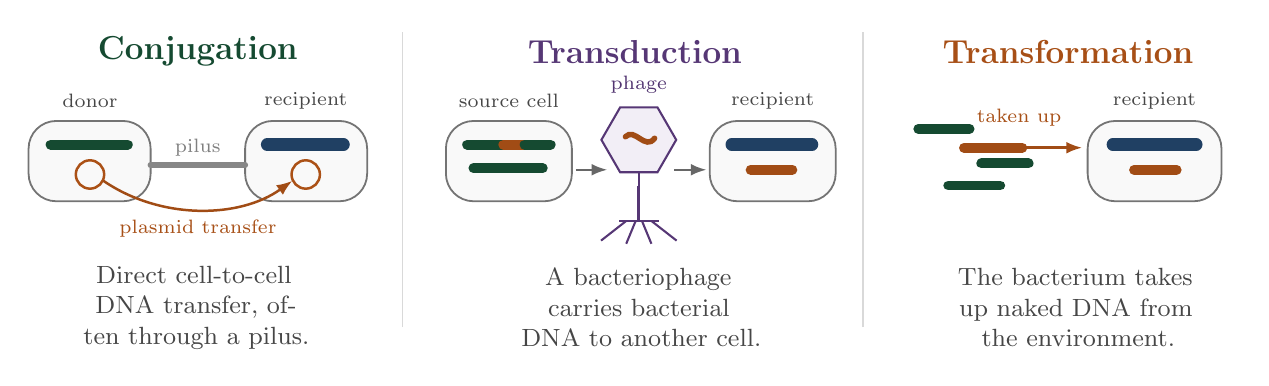
\begin{tikzpicture}[
  scale=1.0,
  paneltitle/.style={font=\bfseries\large},
  note/.style={font=\small,align=center,text width=3.95cm,text=darkgray},
  smallnote/.style={font=\scriptsize,align=center,text=darkgray},
  cell/.style={rounded corners=10pt,draw=darkgray!75,fill=gray!5,line width=.65pt},
  dnaBlue/.style={line width=4.5pt,line cap=round,draw=mainblue!75!black},
  dnaOrange/.style={line width=3.6pt,line cap=round,draw=burntorange!85!black},
  dnaGreen/.style={line width=3.6pt,line cap=round,draw=deepgreen!70!black},
  arrow/.style={-{Latex[length=2mm]},line width=.85pt,draw=darkgray!82},
  transferarrow/.style={-{Latex[length=2mm]},line width=.9pt,draw=burntorange!85!black},
  pilus/.style={line width=2.2pt,draw=darkgray!65,line cap=round},
  phagepart/.style={draw=violet!78!black,line width=.75pt},
  phagefill/.style={draw=violet!78!black,fill=violet!9,line width=.75pt}
]

\begin{scope}
  \node[paneltitle,text=deepgreen!70!black] at (2.25,3.60)
    {Conjugation};

  \draw[cell] (0.10,1.70) rectangle (1.65,2.72);
  \draw[cell] (2.85,1.70) rectangle (4.40,2.72);

  \node[smallnote] at (0.88,2.98) {donor};
  \node[smallnote] at (3.62,2.98) {recipient};

  \draw[dnaGreen] (0.38,2.42)--(1.36,2.42);
  \draw[draw=burntorange!90!black,line width=.9pt]
    (0.88,2.04) circle[radius=.18];

  \draw[dnaBlue] (3.13,2.42)--(4.10,2.42);
  \draw[draw=burntorange!90!black,line width=.9pt]
    (3.62,2.04) circle[radius=.18];

  \draw[pilus] (1.65,2.16)--(2.85,2.16);
  \draw[transferarrow]
    (1.05,1.96).. controls (1.78,1.46) and (2.78,1.48).. (3.45,1.96);

  \node[smallnote,text=gray] at (2.25,2.38)
    {pilus};
  \node[smallnote,text=burntorange!88!black] at (2.25,1.35)
    {plasmid transfer};

  \node[note] at (2.20,0.35)
    {Direct cell-to-cell DNA transfer, often through a pilus.};
\end{scope}

\draw[gray!30,line width=.6pt] (4.85,0.10)--(4.85,3.85);

\begin{scope}[xshift=5.35cm]
  \node[paneltitle,text=violet!78!black] at (2.45,3.60)
    {Transduction};

  \draw[cell] (0.05,1.70) rectangle (1.65,2.72);
  \draw[cell] (3.40,1.70) rectangle (5.00,2.72);

  \node[smallnote] at (0.85,2.98) {source cell};
  \node[smallnote] at (4.20,2.98) {recipient};

  \draw[dnaGreen]  (0.32,2.42)--(0.78,2.42);
  \draw[dnaOrange] (0.78,2.42)--(1.05,2.42);
  \draw[dnaGreen]  (1.05,2.42)--(1.38,2.42);
  \draw[dnaGreen]  (0.40,2.12)--(1.28,2.12);


  \coordinate (ph) at (2.50,2.48);

  \node[
    regular polygon,
    regular polygon sides=6,
    minimum size=9.5mm,
    phagefill
  ] at (ph) {};

  \draw[dnaOrange,line width=2.0pt]
    ($(ph)+(-0.17,0.04)$) .. controls ($(ph)+(-0.05,0.16)$) and ($(ph)+(0.08,-0.14)$) .. ($(ph)+(0.20,0.02)$);

  \draw[phagepart] ($(ph)+(0,-0.42)$)--($(ph)+(0,-0.58)$);
  \draw[phagepart,line width=1.15pt] ($(ph)+(0,-0.58)$)--($(ph)+(0,-1.03)$);
  \draw[phagepart] ($(ph)+(-0.25,-1.03)$)--($(ph)+(0.25,-1.03)$);

  \draw[phagepart] ($(ph)+(-0.16,-1.03)$)--($(ph)+(-0.48,-1.28)$);
  \draw[phagepart] ($(ph)+(-0.04,-1.03)$)--($(ph)+(-0.16,-1.32)$);
  \draw[phagepart] ($(ph)+(0.04,-1.03)$)--($(ph)+(0.16,-1.32)$);
  \draw[phagepart] ($(ph)+(0.16,-1.03)$)--($(ph)+(0.48,-1.28)$);

  \node[smallnote,text=violet!75!black] at (2.50,3.18)
    {phage};

  \draw[arrow] (1.70,2.10)--(2.10,2.10);
  \draw[arrow] (2.95,2.10)--(3.36,2.10);

  \draw[dnaBlue] (3.68,2.42)--(4.70,2.42);
  \draw[dnaOrange] (3.92,2.10)--(4.45,2.10);

  \node[note] at (2.50,0.35)
    {A bacteriophage carries bacterial DNA to another cell.};
\end{scope}

\draw[gray!30,line width=.6pt] (10.70,0.10)--(10.70,3.85);

\begin{scope}[xshift=11.20cm]
  \node[paneltitle,text=burntorange!88!black] at (2.10,3.60)
    {Transformation};

  \draw[cell] (2.35,1.70) rectangle (4.05,2.72);

  \node[smallnote] at (3.20,2.98) {recipient};
  \draw[dnaBlue] (2.67,2.42)--(3.73,2.42);

  \draw[dnaGreen]  (0.20,2.62)--(0.85,2.62);
  \draw[dnaGreen]  (0.58,1.90)--(1.24,1.90);
  \draw[dnaGreen]  (1.00,2.18)--(1.60,2.18);
  \draw[dnaOrange] (0.78,2.38)--(1.52,2.38);

  \node[smallnote,text=burntorange!88!black] at (1.48,2.76)
    {taken up};

  \draw[transferarrow] (1.55,2.38)--(2.28,2.38);

  \draw[dnaOrange] (2.94,2.10)--(3.48,2.10);

  \node[note] at (2.20,0.35)
    {The bacterium takes up naked DNA from the environment.};
\end{scope}

\end{tikzpicture}
\end{document}
